\documentclass[oneside, 11 pt]{report}
\usepackage{hyperref, graphicx}
\title{Operating System}
\date{\today}
\author{NU Rubel \\ \href{mailto:nurubel70@gmail.com}{nurubel70@gmail.com}}
\begin{document}
\maketitle

\section*{Introduction}
An operating system (OS) is system software that manages computer hardware, software resources, and provides common services for computer programs.

Time-sharing operating systems schedule tasks for efficient use of the system and may also include accounting software for cost allocation of processor time, mass storage, printing, and other resources.

For hardware functions such as input and output and memory allocation, the operating system acts as an intermediary between programs and the computer hardware,[1][2] although the application code is usually executed directly by the hardware and frequently makes system calls to an OS function or is interrupted by it. Operating systems are found on many devices that contain a computer – from cellular phones and video game consoles to web servers and supercomputers.

The dominant desktop operating system is Microsoft Windows with a market share of around 82.74\%. macOS by Apple Inc. is in second place (13.23\%), and the varieties of Linux are collectively in third place (1.57\%). In the mobile (including smartphones and tablets) sector, Google Android's share is up to 70\% in the year 2017.[4] According to third quarter 2016 data, Android's share on smartphones is dominant with 87.5 percent with also a growth rate of 10.3 percent per year, followed by Apple's iOS with 12.1 percent with per year decrease in market share of 5.2 percent, while other operating systems amount to just 0.3 percent. Linux distributions are dominant in the server and supercomputing sectors. Other specialized classes of operating systems, such as embedded and real-time systems, exist for many applications.

\tableofcontents

\section{Type of operating system}
	
1.1	Single-tasking and multi-tasking\\
1.2	Single- and multi-user\\
1.3	Distributed\\
1.4	Templated\\
1.5	Embedded\\
1.6	Real-time\\
1.7	Library\\
\section{History}

2.1	Mainframes\\
2.2	Microcomputers\\
\section{Examples}

3.1	Unix and Unix-like operating systems
3.1.1	BSD and its descendants
3.1.2	macOS
3.1.3	Linux
3.2	Microsoft Windows
3.3	Other
\section{Components}

4.1	Kernel
4.1.1	Program execution
4.1.2	Interrupts
4.1.3	Modes
4.1.4	Memory management
4.1.5	Virtual memory
4.1.6	Multitasking
4.1.7	Disk access and file systems
4.1.8	Device drivers
4.2	Networking
4.3	Security
4.4	User interface
4.4.1	Graphical user interfaces
\section{Real-time operating systems}
Main article: Real-time operating system
A real-time operating system (RTOS) is an operating system intended for applications with fixed deadlines (real-time computing). Such applications include some small embedded systems, automobile engine controllers, industrial robots, spacecraft, industrial control, and some large-scale computing systems.

An early example of a large-scale real-time operating system was Transaction Processing Facility developed by American Airlines and IBM for the Sabre Airline Reservations System.

Embedded systems that have fixed deadlines use a real-time operating system such as VxWorks, PikeOS, eCos, QNX, MontaVista Linux and RTLinux. Windows CE is a real-time operating system that shares similar APIs to desktop Windows but shares none of desktop Windows' codebase.[33] Symbian OS also has an RTOS kernel (EKA2) starting with version 8.0b.

Some embedded systems use operating systems such as Palm OS, BSD, and Linux, although such operating systems do not support real-time computing.
\section{Operating system development as a hobby}
See also: Hobbyist operating system development
Operating system development is one of the most complicated activities in which a computing hobbyist may engage.[citation needed] A hobby operating system may be classified as one whose code has not been directly derived from an existing operating system, and has few users and active developers.[34]

In some cases, hobby development is in support of a "homebrew" computing device, for example, a simple single-board computer powered by a 6502 microprocessor. Or, development may be for an architecture already in widespread use. Operating system development may come from entirely new concepts, or may commence by modeling an existing operating system. In either case, the hobbyist is his/her own developer, or may interact with a small and sometimes unstructured group of individuals who have like interests.

Examples of a hobby operating system include Syllable and TempleOS.
\section{Diversity of operating systems and portability}
Application software is generally written for use on a specific operating system, and sometimes even for specific hardware.[citation needed] When porting the application to run on another OS, the functionality required by that application may be implemented differently by that OS (the names of functions, meaning of arguments, etc.) requiring the application to be adapted, changed, or otherwise maintained.

Unix was the first operating system not written in assembly language, making it very portable to systems different from its native PDP-11.[35]

This cost in supporting operating systems diversity can be avoided by instead writing applications against software platforms such as Java or Qt. These abstractions have already borne the cost of adaptation to specific operating systems and their system libraries.

Another approach is for operating system vendors to adopt standards. For example, POSIX and OS abstraction layers provide commonalities that reduce porting costs.\\
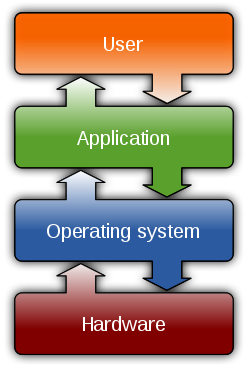
\includegraphics[width = 170 pt]{img.jpg}


\end{document}